\section{System Design and Prototyping}
\label{sec:syst-design-prot}

This section describes the design and implementation of our prototype system. We start by summarizing the design considerations in this head-orientation targeting, and for each consideration, we make the choice of commercial off-the-shelf (COTS) components. Afterwards, we conclude this section by a depiction of the overall system architecture that is used for both our study and future application development. 

\subsection{Design Considerations}
\label{sec:design-cons}

To effectively enables the physical targeting based on user's head movement, and build such a platform for applications, we have come up with the following design considerations and the justification for each.

{\bf Directional area selection:} To be aligned with the user's head orientation, the sensing modality should be directional. Merely direction is not enough, from Section~\ref{sec:background}, the head muscle's fundamental limitation and Fitts' law imposes us to choose an area selection technique. However,  with a larger coverage area, there will be a higher chance for disambiguation. We should find the proper technique that achieves area selection while still providing ways for a more fine-grained resolution.

% the two visual feedback seems a bit random...
{\bf Leverage visual feedback:} Since the user cannot see his own head orientation, there should be some effective ways to provide feedback to the users. We consider two types of visual feedbacks. The first comes from the environment which enables instantaneous visual cue while the user is looking around. The second should remain unchanged even if the users' head orientation has changed; in such a way, further interactions are enabled without imposing the burden of staring. But such a display shouldn't distract the user's current line-of-sight attention -- which means a near-eye display is better than using a hand-held device. 

% A calmer~\cite{weiser_coming_1997} approach is to locate visual feedback about selection targets in the environment, to prevent distraction and interruption. Such feedback should be delivered instantaneously, while users look around a room.

{\bf Flexible communication:} The system is for the interaction with the environment, therefore the communication among devices should be flexible. Especially there would be a consensus problem if the end-nodes are not agreeing on what the user is looking at. The communication would be necessary for resolving the inconsistency in such a distributed environment. Also providing a flexible communication capability can make the system as a platform for other applications. 

{\bf Adjustable angle:} From our pilot study, we have learned that human's head orientation pointing is biased for each person. In order to align area selection technique, there should be ways to adjust or calibrate the covered area.

These design considerations find their expression in our selection of techniques in the following few subsections.

\subsection{IR as beam cursor}
\label{sec:ir-as-beam}

For the directional area selection technique, we have chosen to use infrared (IR) for a couple of reasons.  

First, the signal characteristics of IR makes it suitable for directional area selection. There are a wide range of viewing angles that we can choose (DigiKey offers IR emitters from $4^\circ$ to $240^\circ$, however, most are around $20^\circ$ of viewing angle). This leads to a cone shape-like area coverage and can be well-aligned with human's line of sight. 

Second, for the disambiguation consideration, since the infrared illuminance falls off with respect to both the offset angle from the center and the distance to the emitter, even though the signal might cover multiple targets, using the intensity from the receivers can help disambiguation.  
% for the 4 degree to 240 degree, I used information from http://www.digikey.com/product-search/en/optoelectronics/infrared-uv-visible-emitters/524328?k=IR

In addition, IR has been used for remote control for many years. The emitters and receivers are fairly cheap to manufacture; and it's easy for integration with existing devices. 
What's more, IR is immune to most interference sources. The ambient IR might influence the IR receivers' intensity reading, however with simple IR signal validation, the receiver is still safe. There might be issues for signal reflection, either bouncing from the ground to the target or bouncing back to the opposite direction. However, such visual feedback is not aligned with the user's attention so no further action from the user might be taken; or the genuine target could easily beat the false positive since the one with reflection tends to travel a longer distance, making the signal strength smaller.

Therefore, we can attach an IR emitter to capture the head orientation and install some IR receivers in the environment for both signals detection and intensity reading. For our prototype, we have found some COTS components for IR. 
The IR emitter is the one from OSRAM Opto Semiconductors Inc with manufacturer part number SFH 4545. From the data-sheet, it has a view angle of $10^\circ$. Part of the reason we have chosen it is because the radiant intensity can quite high if we provide it with sufficient current flow (550mW/sr @ 100mA). We can then easily adjust it using a resistor to satisfy different demands. 
% transmitter webpage: http://www.digikey.com/product-search/en?x=0&y=0&lang=en&site=us&KeyWords=475-2919-ND
For the IR receiver, we use 38.0kHz IR Receiver Modules from Vishay Semiconductor Opto Division (manufacturer part number TSOP38238). 
% receiver webpage http://www.digikey.com/product-detail/en/TSOP38238/751-1227-ND/1681362
In order to read the IR intensity, we integrates another IR light-to-voltage converter from AMS-TAOS USA Inc (manufacturer part number TSL267-LF) which is pretty sensitive to IR irradiance. 
% http://www.digikey.com/product-detail/en/TSL267-LF/TSL267-LF-ND/3095052

We use Arduino platform for the prototyping, and there is an easy-to-use IR library\footnote{\url{https://github.com/shirriff/Arduino-IRremote}} where we can customize the IR signal for both transmission and reception. To read the IR intensity, an 10-bit ADC is attached to the output of TSL267-LF which gives a reading from 0 to 1023. 

\subsection{Environment LEDs and Head-up display}
\label{sec:head-up-display}
As we have argued for the visual feedback design considerations, the environment should provide instantaneous visual cue to respond to user's head orientation. This can be easily achieved with 1-bit LEDs on each devices that has an IR receiver. For the visual feedback that is persistent even when the user's head orientation has changed, we have considered a few COTS solutions that support the head-up display, and ended up with Google Glass because it's easy to program (it supports standard Android programming) and the device is also light-weight for everyday use. At the time of writing, we have Google Glass running Android 4.0.4 (software version: XE12). 

\subsection{Wireless Communication}
\label{sec:wirel-comm}

There are many choices of wireless communication techniques that we could consider to accompany IR's directional targeting. WiFi, Bluetooth Low Energy (BLE) and 802.15.4 (ZigBee) radio are all candidates for such communications. A detailed comparison is out of the scope of this paper. For our prototype, we have chosen to use XBee ZB\footnote{XBee: http://www.digi.com/xbee/}(based on ZigBee protocol and 802.15.4 radio) for the mesh network because of the ease to program and integration to Arduino platform. The COTS adapter provides an easy-to-use interface where we could use either hardware serial pins or the software serial library to send and receive messages. 

As we mentioned that the communication capability has to be included to resolve the consensus view of head orientation, we use the star topology -- the node which controls IR emission acts as the PAN coordinator. It collects the IR received signal strength (RSS) from each targets and runs a local algorithm to determine which one is the current target. 

Using such an architecture for communication also makes the integration with Google Glass easier. For now, Google Glass is only capable of WiFi and Bluetooth; so we have to add a Bluetooth modem to establish connections with Google Glass\footnote{This is a compromise now, and we are planning to migrate the entire system to BLE once Google upgrade the Glass software to Android 4.4+. The prototype now suffice our demand to run the head orientation study.}. We use BlueSMiRF Silver (WRL-12577) for our prototype. 

\subsection{3D Printed Adjustable Holder}
\label{sec:3d-print-adjust}
To compensate for the bias of each person's line of sight with the IR emitter, we have designed the holder that can be easily attached onto Google Glass while we can adjust the beam angle flexibly.

\begin{figure}[t]
\centering
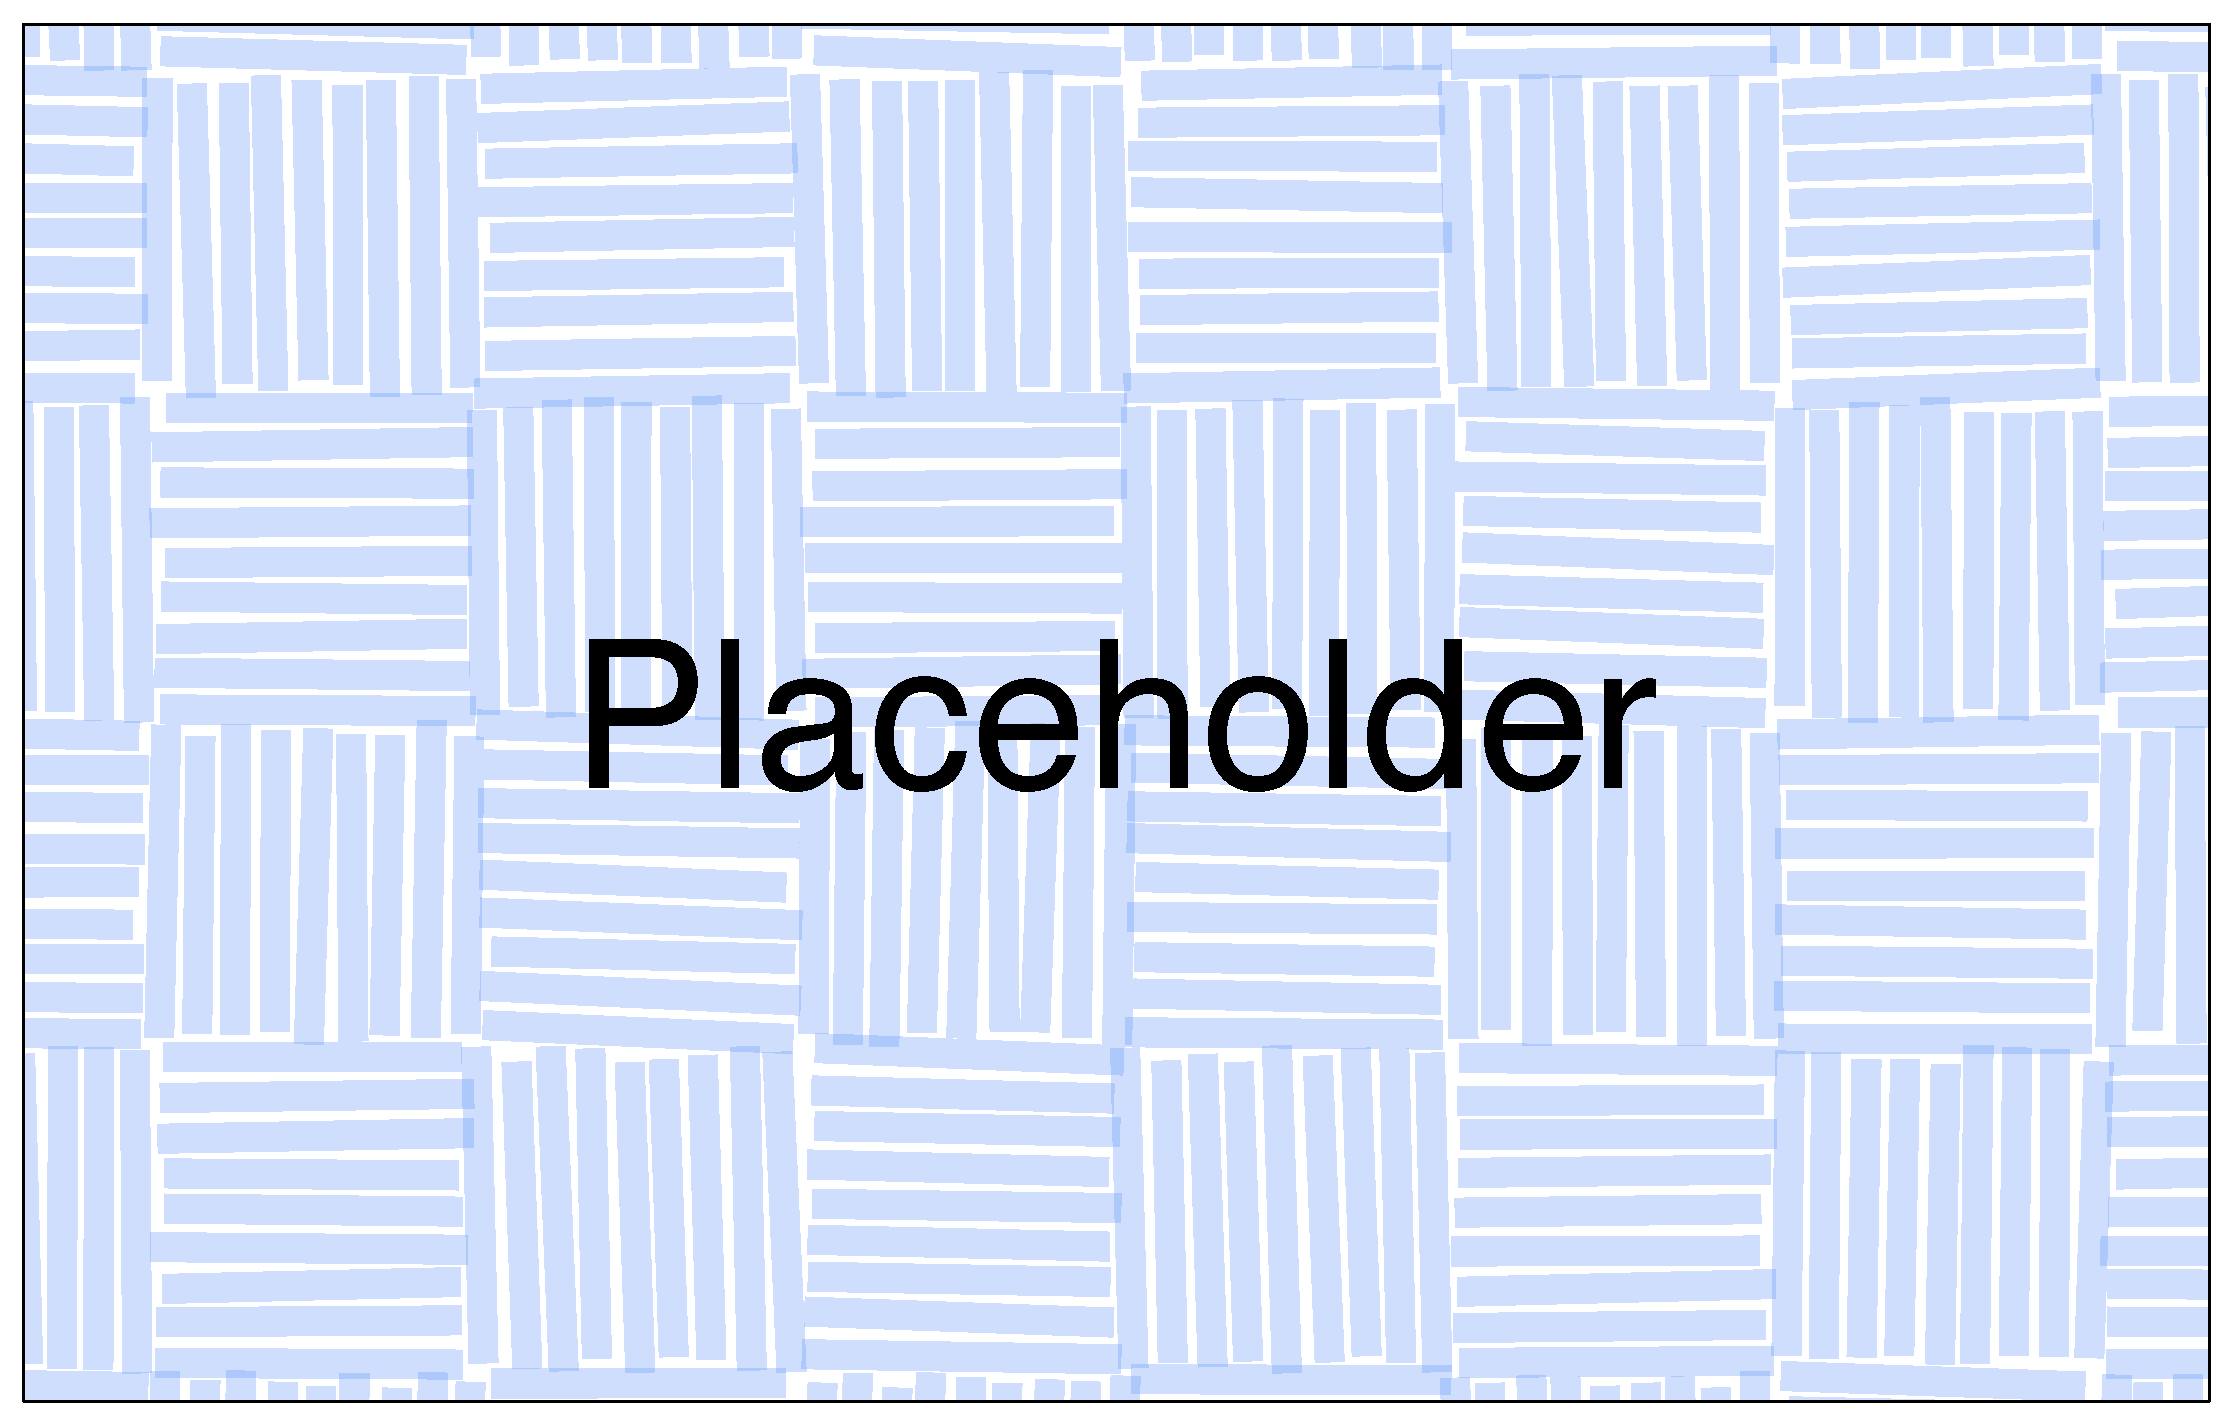
\includegraphics[width=0.9\columnwidth]{figures/placeholder.pdf}
\caption{we should replace this place-holder with Claire's design and printed version.}
\label{fig:3d-holder}
\end{figure}

\subsection{Overall System}
\label{sec:overall-system}
So far we have been discussing separate components that fit our design considerations. To stitch them into a single system, we use the following architecture shown in Figure~\ref{fig:architecture}.

\begin{figure}[t]
\centering
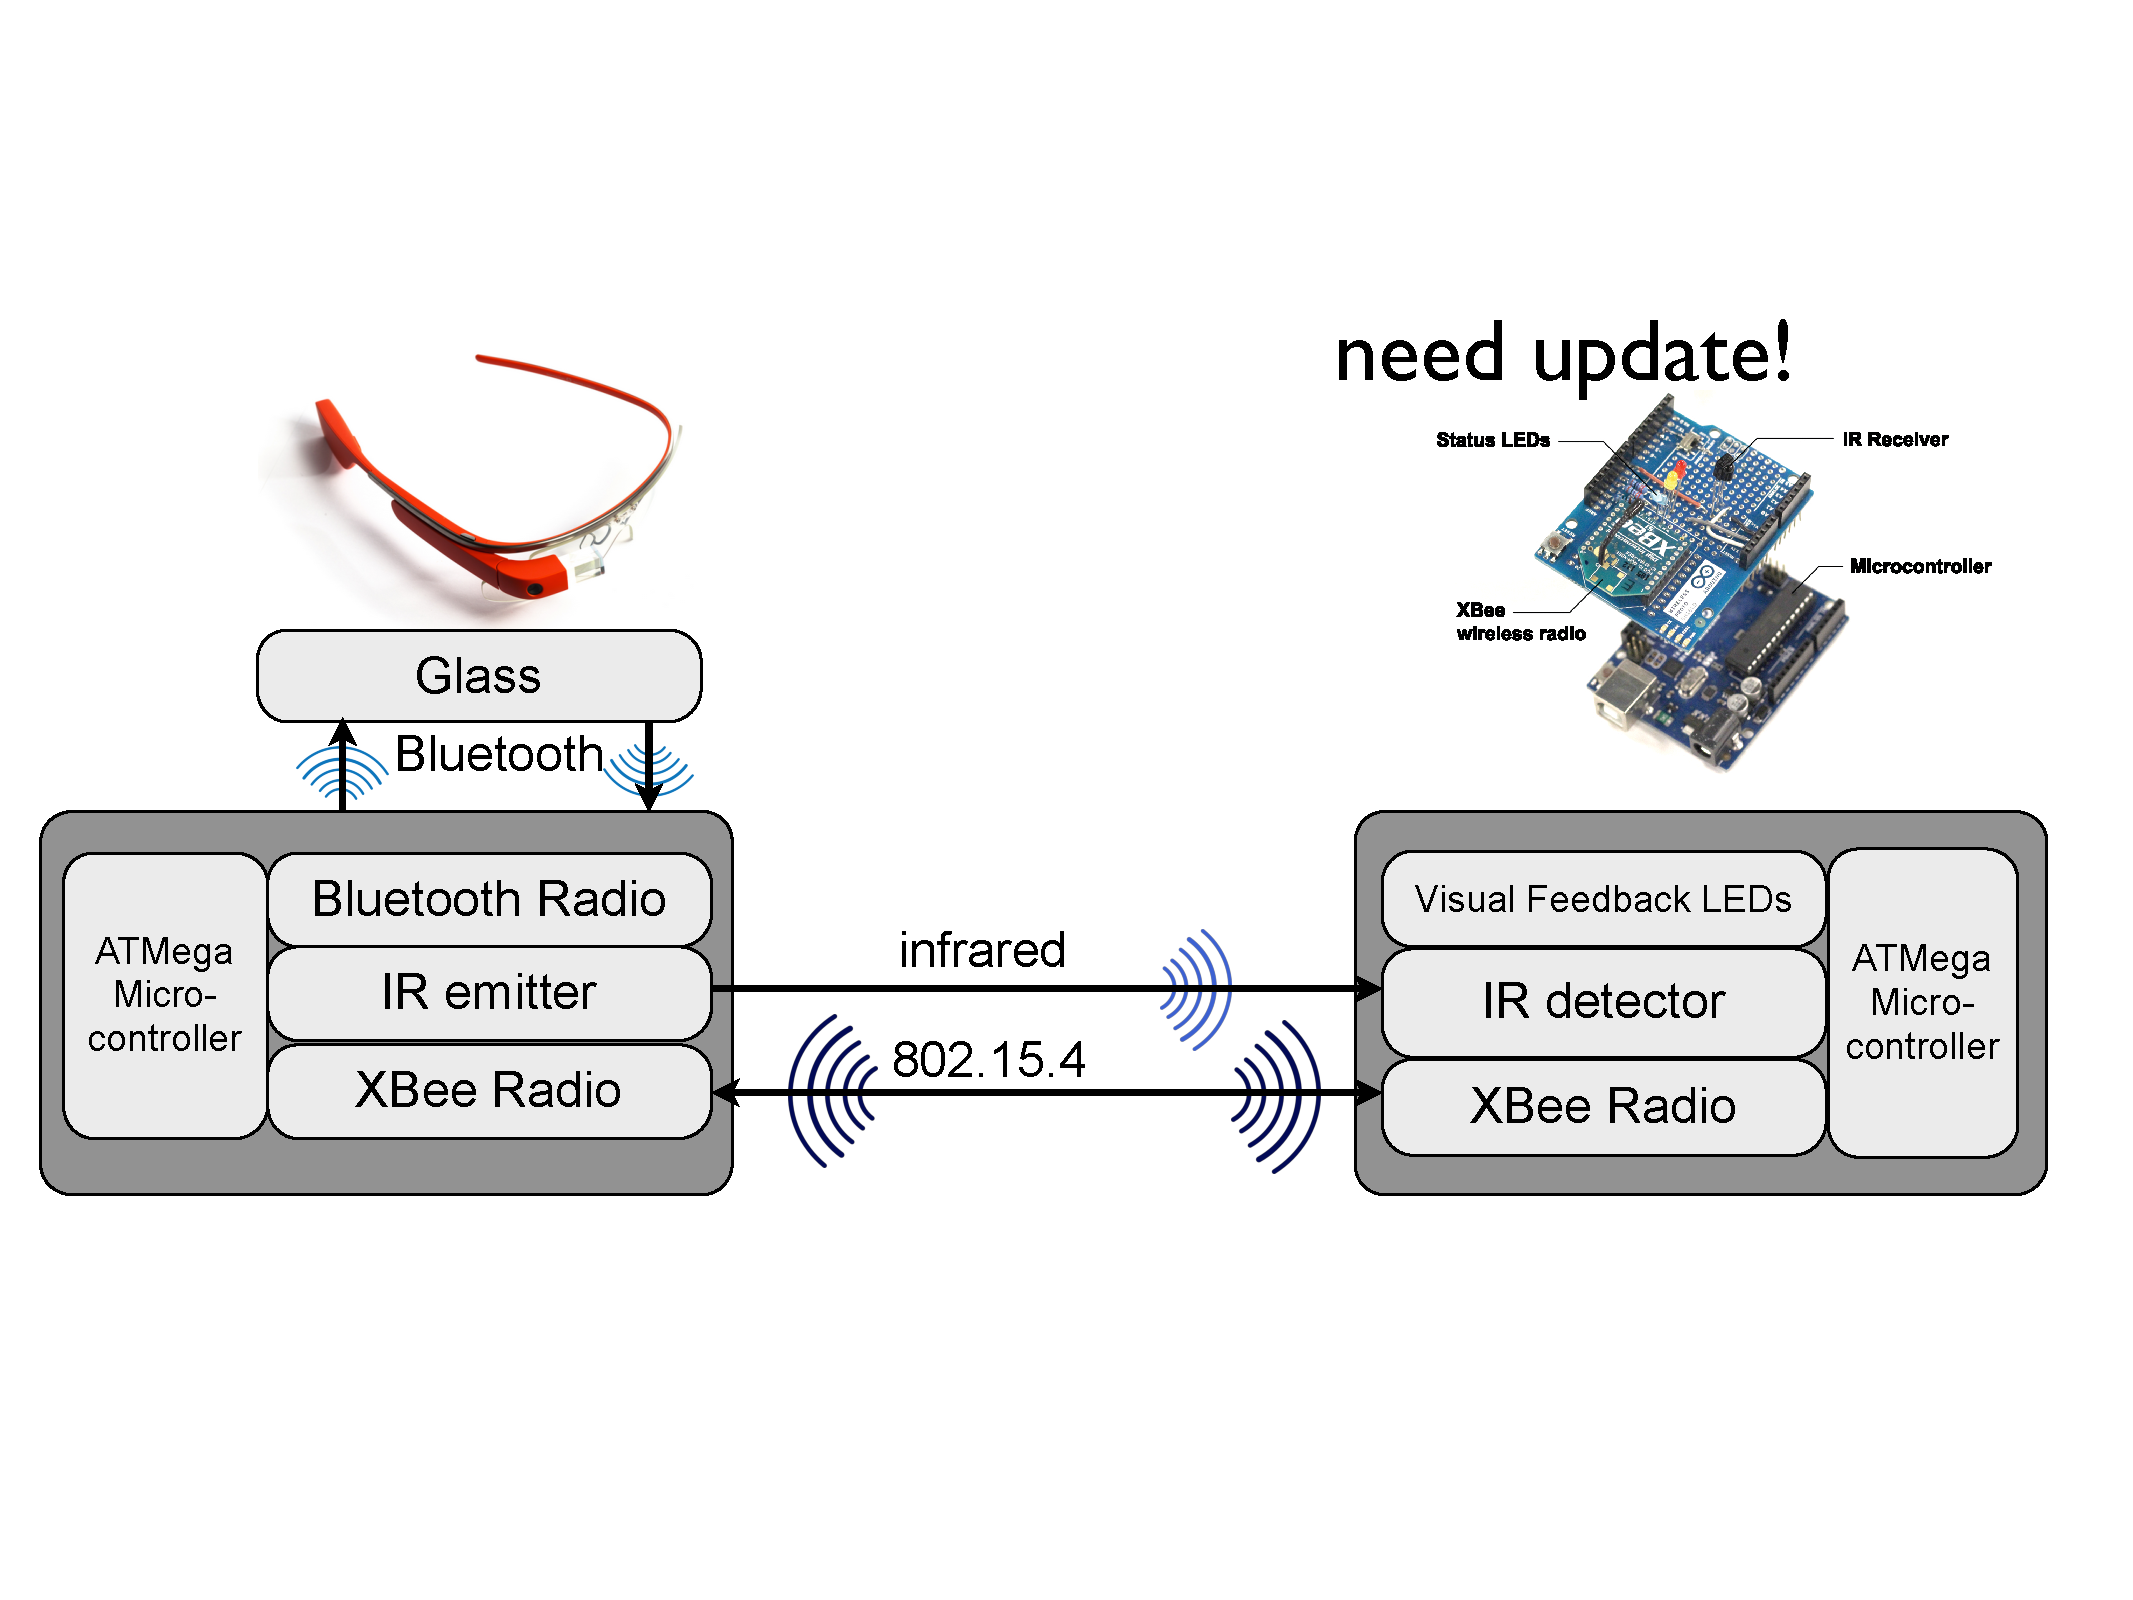
\includegraphics[width=0.9\columnwidth]{figures/architecture.pdf}
\caption{In our system architecture, targeting is captured by IR signal but the confirmation and coordination is over 802.15.4. Google Glass communicates with the system through Bluetooth.}
\label{fig:architecture}
\end{figure}

\ben{this paragraph needs refinement. Maybe a good idea is to use one single sentence to summarize the disambiguation and say we will talk about it in the next section.}
In our system, the microcontroller at the Google Glass side (we will call it the master) takes charge of bridging the end nodes and the Glass. It constantly transmits IR signal no specific connection with any node has been established. When the node receives such signal, they validate the packet and send back IR intensity readings. The master may simply use the IR intensity changes to determine which is the intended targets, or pass the information to Google Glasss where the Glass combines both motion sensor readings with the IR signal intensity to disambiguate. We will leave the algorithm description in the next section. Once a decision has been made, such information will be sent back to the node and the visual feedback is provided to the user. The user is free to adjust during the targeting process, our algorithm will dynamically adjust to the user's head movement. Once the user confirms the targeting, he could easily tap the touchpad. Single tap only enables highlighting, targeting confirmation is done with a second tap. This is the last resort for the user to adjust targets. Since the disambiguation matters to the overall performance, we will focus on the discussion in the next section.

%%% Local Variables: 
%%% mode: latex
%%% TeX-master: "uist14"
%%% End: 
